\documentclass[tikz,border=3pt]{standalone}
\usepackage[utf8]{inputenc}
\usepackage[T1]{fontenc}
\usepackage{lmodern}
\renewcommand{\familydefault}{\sfdefault}
\usepackage{sansmath}\sansmath
\usepackage{chemfig}
\usepackage{pgfplots}\pgfplotsset{compat=1.18,/pgf/number format/use comma,/pgf/number format/1000 sep={.}}
\usetikzlibrary{arrows.meta,calc,positioning,decorations.pathmorphing,patterns}
% paleta del sitio
\definecolor{nar}{HTML}{E8680C}\definecolor{narc}{HTML}{FFB35C}\definecolor{hielo}{HTML}{FFF3E8}
\definecolor{tinta}{HTML}{1D1D1F}\definecolor{gris}{HTML}{6E6E73}\definecolor{lila}{HTML}{7C5CF0}
\definecolor{azul}{HTML}{2F6FD6}\definecolor{menta}{HTML}{17A673}\definecolor{coral}{HTML}{E8342A}
\begin{document}
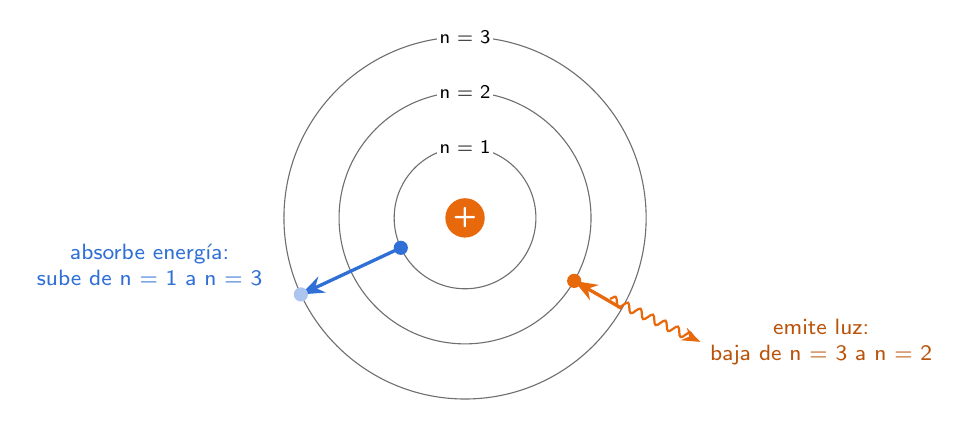
\begin{tikzpicture}[font=\small]
\draw[gris] (0,0) circle (0.9);
\draw[gris] (0,0) circle (1.6);
\draw[gris] (0,0) circle (2.3);
\fill[nar] (0,0) circle (0.25); \node[text=white,font=\bfseries] at (0,0) {+};
\node[font=\scriptsize,fill=white,inner sep=1pt] at (0,0.9) {n = 1};
\node[font=\scriptsize,fill=white,inner sep=1pt] at (0,1.6) {n = 2};
\node[font=\scriptsize,fill=white,inner sep=1pt] at (0,2.3) {n = 3};
\draw[azul,very thick,-{Stealth}] (-0.816,-0.38) -- (-2.085,-0.972);
\fill[azul] (-0.816,-0.38) circle (0.09);
\fill[azul!40] (-2.085,-0.972) circle (0.09);
\node[anchor=east,align=center,font=\footnotesize,text=azul] at (-2.45,-0.6) {absorbe energía:\\sube de n = 1 a n = 3};
\draw[nar,very thick,-{Stealth}] (1.992,-1.15) -- (1.386,-0.8);
\fill[nar] (1.386,-0.8) circle (0.09);
\draw[nar,thick,decorate,decoration={snake,amplitude=1.5pt,segment length=5pt,post length=3pt},-{Stealth}] (1.839,-1.025) -- (2.989,-1.575);
\node[anchor=west,align=center,font=\footnotesize,text=nar!80!black] at (2.989,-1.575) {emite luz:\\baja de n = 3 a n = 2};

\end{tikzpicture}
\end{document}
